\documentclass{article}
\usepackage[T1]{fontenc}
\usepackage{lmodern}
\usepackage{graphicx}
\usepackage{amsmath,amssymb}
\usepackage[a4paper,margin=2cm]{geometry}
\usepackage[absolute,overlay]{textpos}
\setlength{\TPHorizModule}{1mm}
\setlength{\TPVertModule}{1mm}
\usepackage[indonesian]{babel}
\usepackage{hyperref}
\setlength{\emergencystretch}{2em}
% unit: Halaman 84

\begin{document}

% === Halaman 84 (llm) ===

\begin{itemize}
  \item \textit{Column round} menerapkan $\text{QR}(a, b, c, d)$ kepada tiap kolom matriks $\text{state } 4\times 4$, sedangkan \textit{row round} menerapkannya kepada tiap baris matriks.
\end{itemize}

\vspace{53.46mm}

\noindent // Column round
\[
\begin{aligned}
\text{QR}(0, 4, 8, 12) & \quad // \text{ kolom 1} \\
\text{QR}(5, 9, 13, 1) & \quad // \text{ kolom 2} \\
\text{QR}(10, 14, 2, 6) & \quad // \text{ kolom 3} \\
\text{QR}(15, 3, 7, 11) & \quad // \text{ kolom 4}
\end{aligned}
\]

\vspace{10mm}

\noindent // Row round
\[
\begin{aligned}
\text{QR}(0, 1, 2, 3) & \quad // \text{ baris 1} \\
\text{QR}(5, 6, 7, 4) & \quad // \text{ baris 2} \\
\text{QR}(10, 11, 8, 9) & \quad // \text{ baris 3} \\
\text{QR}(15, 12, 13, 14) & \quad // \text{ baris 4}
\end{aligned}
\]

% deskripsi: Matriks state 4x4 yang berisi angka 0 sampai 15
% bbox normalisasi: [0.7500, 0.2600, 0.9100, 0.5500]
\begin{textblock*}{33.60mm}(157.50mm,77.22mm)
\noindent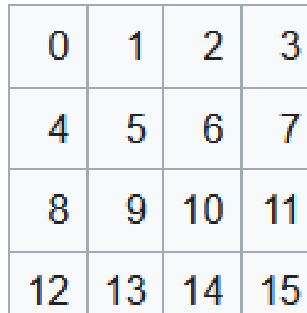
\includegraphics[width=33.60mm,height=86.13mm]{../../images/llm/page_084_img_01.png}%
\end{textblock*}

% deskripsi: Definisi algoritma QR(a, b, c, d) dengan operasi XOR dan rotasi
% bbox normalisasi: [0.4700, 0.2800, 0.7000, 0.4600]
\begin{textblock*}{48.30mm}(98.70mm,83.16mm)
\noindent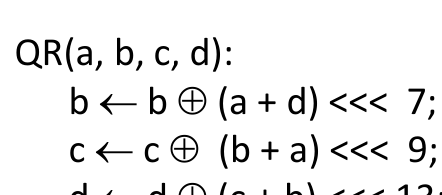
\includegraphics[width=48.30mm,height=53.46mm]{../../images/llm/page_084_img_02.png}%
\end{textblock*}

% deskripsi: Implementasi C++ makro untuk ROTL dan QR
% bbox normalisasi: [0.4700, 0.6500, 0.8100, 0.9200]
\begin{textblock*}{71.40mm}(98.70mm,193.05mm)
\noindent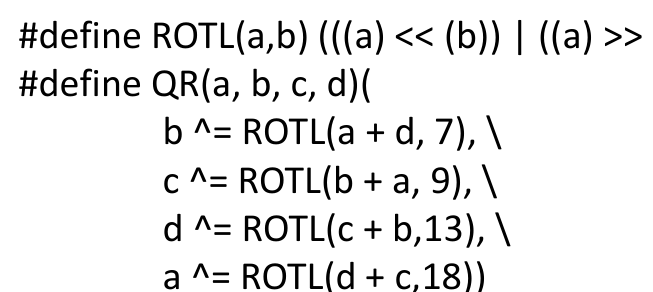
\includegraphics[width=71.40mm,height=80.19mm]{../../images/llm/page_084_img_03.png}%
\end{textblock*}

\end{document}
